\documentclass[11pt,xcolor=dvipsnames,compress,aspectratio=169]{beamer}
\usetheme{Warsaw}
\usecolortheme{beaver}
\usepackage[latin1]{inputenc}
\usepackage{amssymb,amsmath,mathrsfs}
\usepackage{amsthm}
\usepackage{natbib}
\usepackage{enumerate}
\usepackage{color}
\usepackage{upgreek}
\usepackage{wrapfig}
\usepackage{subcaption}
\usepackage{textpos}
\usepackage{multimedia}
\usepackage{colortbl}
\usepackage[makeroom]{cancel}
\usepackage{array}
\usepackage{overpic,tikz}
\usepackage{tcolorbox}
\usepackage{multirow}
\usepackage{amssymb,amsmath,mathrsfs,bbold,dsfont}
\usepackage[makeroom]{cancel}
\usepackage{graphicx}
\usepackage{rotating}
\beamertemplatenavigationsymbolsempty
\everymath{\displaystyle}
%%%%%%%%%%%%%%%%%%%%%%%%%%%%%%%%%%%%%%%%%%%%%%%%%%%%%%%%%%%%%%%%%%%%%%%%%%%%%%%%%%%%%%%%%%%%%%%%%%%%
\title{Forward Model}
\author{CCO}
\institute{{Institute for Computational Engineering and Sciences\\Center of Computational Oncology\\The University of Texas at Austin}}
\date{\today}
%%%%%%%%%%%%%%%%%%%%%%%%%%%%%%%%%%%%%%%%%%%%%%%%%%%%%%%%%%%%%%%%%%%%%%%%%%%%%%%%%%%%%%%%%%%%%%%%%%%%
\begin{document}
%%%%%%%%%%%%%%%%%%%%%%%%%%%%%%%%%%%%%%%%%%%%%%%%%%%%%%%%%%%%%%%%%%%%%%%%%%%%%%%%%%%%%%%%%%%%%%%%%%%%
\frame{\frametitle{}\titlepage}\logo{}
%%%%%%%%%%%%%%%%%%%%%%%%%%%%%%%%%%%%%%%%%%%%%%%%%%%%%%%%%%%%%%%%%%%%%%%%%%%%%%%%%%%%%%%%%%%%%%%%%%%%
\frame{\frametitle{Treatment model}
\begin{align*}
S_\alpha(D_\alpha,\tau_\alpha,t^*_\alpha)=S_\alpha=D_\alpha \exp(-\tau_\alpha(t-t^*_\alpha))\mathcal{H}(t-t^*_\alpha).
\end{align*}
\begin{itemize}
\item $\alpha=h$ (Trastuzumab) or $\alpha=d$ (Doxorubicin);
\item $D$: drug dose;
\item $\tau$: drug decay;
\item $t^*$: time of the treatment;
\item $\mathcal{H}$: Heaviside function.
\end{itemize}
\begin{align*}
\frac{d T}{d t}&=\underbrace{rT\left(1-\frac{T}{K}\right)}_{\text{logistic growth}}-\underbrace{(\delta_d+\delta_{hd}S_h(\tau_h\alert{+\tau_{dh}S_d(\tau_d)}))S_d(\tau_d)T}_{\text{Doxorubicin treatment}}-\underbrace{\delta_hS_h(\tau_h\alert{+\tau_{dh}S_d(\tau_d)})T}_{\text{Trastuzumab treatment}}.
\end{align*}
}
%%%%%%%%%%%%%%%%%%%%%%%%%%%%%%%%%%%%%%%%%%%%%%%%%%%%%%%%%%%%%%%%%%%%%%%%%%%%%%%%%%%%%%%%%%%%%%%%%%%%
\frame{\frametitle{Treatment model - multiple treatment days}
\begin{align*}
S_\alpha(D_\alpha,\tau_\alpha,t^*_\alpha)=S_\alpha=D_\alpha \exp(-\tau_\alpha(t-t^*_\alpha))\mathcal{H}(t-t^*_\alpha).
\end{align*}
\begin{align*}
\frac{d T}{d t}&=rT\left(1-\frac{T}{K}\right)-(\delta_h\textrm{tras}+\textrm{doxo})T,\\
\textrm{tras}&=\sum_{j=1}^{N_h}S_h\left(\tau_h^j+\tau_{dh}\left(\sum_{i=1}^{N_d}S_d(\tau_d^i)\right)\right)\\
\textrm{doxo}&=\sum_{i=1}^{N_d}(\delta_d+\delta_{hd}\textrm{tras})S_d(\tau_d^i)
\end{align*}
\begin{itemize}
\item $N_d$: Number of Doxorubicin treatments.
\item $N_h$: Number of Trastuzumab treatments.
\end{itemize}
}
%%%%%%%%%%%%%%%%%%%%%%%%%%%%%%%%%%%%%%%%%%%%%%%%%%%%%%%%%%%%%%%%%%%%%%%%%%%%%%%%%%%%%%%%%%%%%%%%%%%%
\frame{\frametitle{Simulations}
\begin{figure}[!htbp]
\centering
\begin{subfigure}[tb]{.49\linewidth}
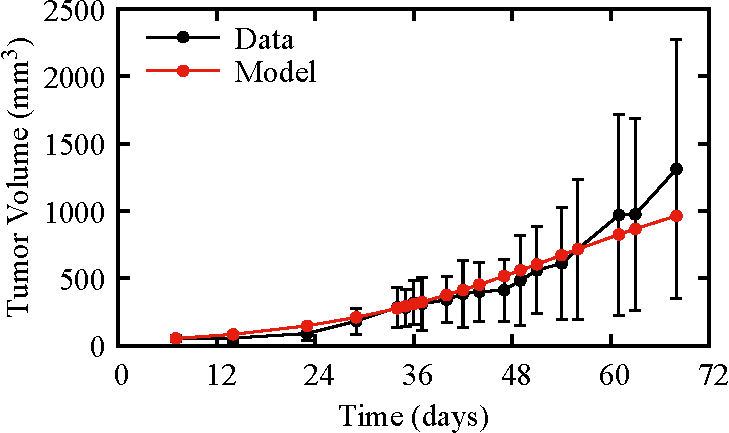
\includegraphics[width=1.0\linewidth]{solution_group_1}
\caption{Group 1}
\end{subfigure}
\begin{subfigure}[tb]{.49\linewidth}
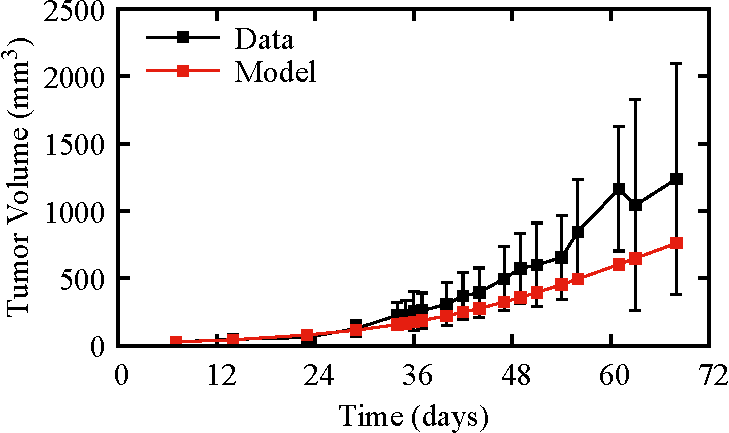
\includegraphics[width=1.0\linewidth]{solution_group_2}
\caption{Group 2}
\end{subfigure}
\end{figure}
}
%%%%%%%%%%%%%%%%%%%%%%%%%%%%%%%%%%%%%%%%%%%%%%%%%%%%%%%%%%%%%%%%%%%%%%%%%%%%%%%%%%%%%%%%%%%%%%%%%%%%
\frame{\frametitle{Simulations}
\begin{figure}[!htbp]
\centering
\begin{subfigure}[tb]{.49\linewidth}
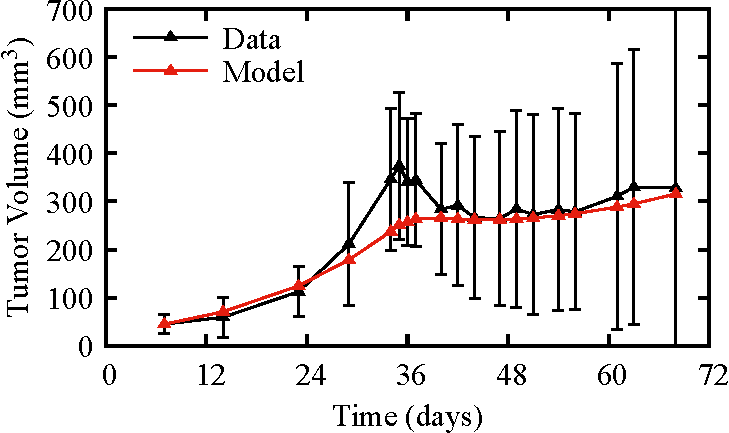
\includegraphics[width=1.0\linewidth]{solution_group_3}
\caption{Group 3}
\end{subfigure}
\begin{subfigure}[tb]{.49\linewidth}
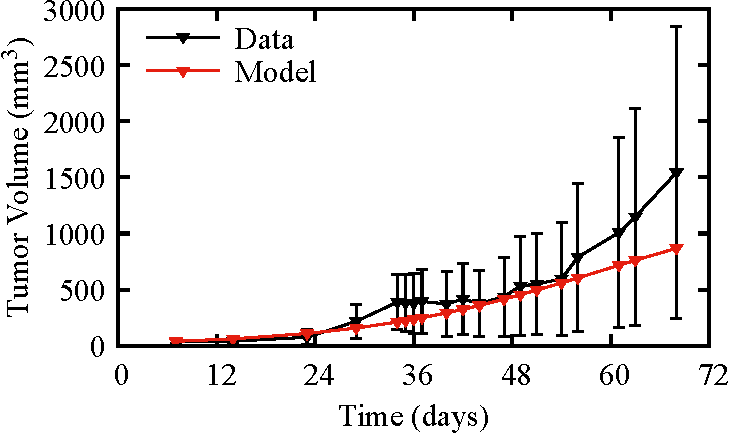
\includegraphics[width=1.0\linewidth]{solution_group_4}
\caption{Group 4}
\end{subfigure}
\end{figure}
}
%%%%%%%%%%%%%%%%%%%%%%%%%%%%%%%%%%%%%%%%%%%%%%%%%%%%%%%%%%%%%%%%%%%%%%%%%%%%%%%%%%%%%%%%%%%%%%%%%%%%
\frame{\frametitle{Simulations}
\begin{figure}[!htbp]
\centering
\begin{subfigure}[tb]{.49\linewidth}
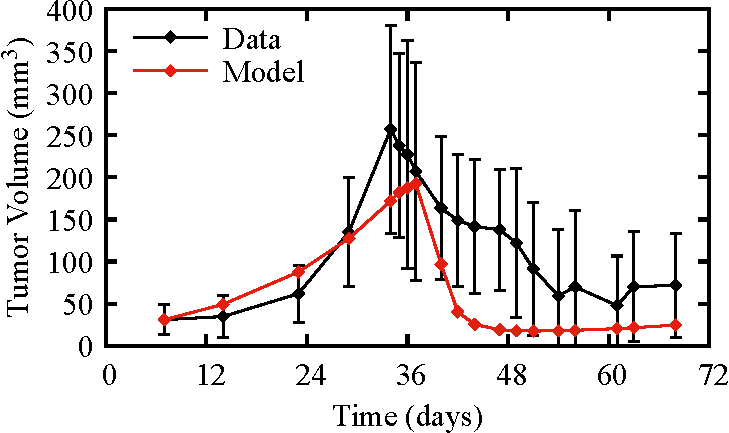
\includegraphics[width=1.0\linewidth]{solution_group_5}
\caption{Group 5}
\end{subfigure}
\begin{subfigure}[tb]{.49\linewidth}
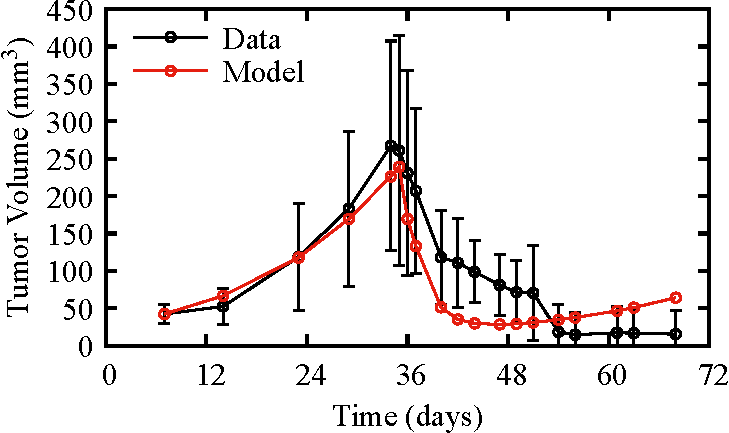
\includegraphics[width=1.0\linewidth]{solution_group_6}
\caption{Group 6}
\end{subfigure}
\end{figure}
}
%%%%%%%%%%%%%%%%%%%%%%%%%%%%%%%%%%%%%%%%%%%%%%%%%%%%%%%%%%%%%%%%%%%%%%%%%%%%%%%%%%%%%%%%%%%%%%%%%%%%
\end{document}
%%%%%%%%%%%%%%%%%%%%%%%%%%%%%%%%%%%%%%%%%%%%%%%%%%%%%%%%%%%%%%%%%%%%%%%%%%%%%%%%%%%%%%%%%%%%%%%%%%%%